% Class Notes Template
\documentclass[12pt]{article}
\usepackage[margin=1in]{geometry} 
\usepackage[utf8]{inputenc}

% Packages
\usepackage[french, english]{babel}
\usepackage{amsmath, amsthm, amssymb ,amsfonts, graphics, tikz, float, enumerate}
\usepackage{listings}
\usepackage{color} %red, green, blue, yellow, cyan, magenta, black, white
\definecolor{mygreen}{RGB}{28,172,0} % color values Red, Green, Blue
\definecolor{mylilas}{RGB}{170,55,241}

\lstset{language=Matlab,%
	%basicstyle=\color{red},
	breaklines=true,%
	morekeywords={matlab2tikz},
	keywordstyle=\color{blue},%
	morekeywords=[2]{1}, keywordstyle=[2]{\color{black}},
	identifierstyle=\color{black},%
	stringstyle=\color{mylilas},
	commentstyle=\color{mygreen},%
	showstringspaces=false,%without this there will be a symbol in the places where there is a space
	numbers=left,%
	numberstyle={\tiny \color{black}},% size of the numbers
	numbersep=9pt, % this defines how far the numbers are from the text
	emph=[1]{for,end,break},emphstyle=[1]\color{blue}, %some words to emphasise
	%emph=[2]{word1,word2}, emphstyle=[2]{style},    
}

% Title
\title{ECON 6130 - Problem Set \# 1}
\date{\today}
\author{Julien Manuel Neves}

% Use these for theorems, lemmas, proofs, etc.
\theoremstyle{definition}
\newtheorem{example}{Example}[section]
\newtheorem{theorem}{Theorem}
\newtheorem{lemma}[theorem]{Lemma}
\newtheorem{proposition}[theorem]{Proposition}
\newtheorem{claim}[theorem]{Claim}
\newtheorem{axiom}[theorem]{Axiom}
\newtheorem{corollary}[theorem]{Corollary}
\newtheorem{remark}[theorem]{Remark}
\newtheorem{definition}[theorem]{Definition}

% Usefuls Macros
\newcommand\N{\mathbb{N}}
\newcommand\E{\mathbb{E}}
\newcommand\R{\mathbb{R}}
\newcommand\F{\mathcal{F}}
\newcommand\Z{\mathbb{Z}}
\newcommand\st{\text{ such that }}
\newcommand\seq[1]{\{ #1 \}}
\newcommand{\inv}{^{-1}}


\newcommand{\norm}[1]{\|#1 \|}
\newcommand{\inp}[2]{\langle #1, #2 \rangle}

\newcommand{\pa}[1]{\left(#1\right)}
\newcommand{\bra}[1]{\left[#1\right]}
\newcommand{\cbra}[1]{\left\{#1\right\}}

\newcommand{\pfrac}[2]{\pa{\frac{#1}{#2}}}
\newcommand{\bfrac}[2]{\bra{\frac{#1}{#2}}}

\newcommand{\mat}[1]{\begin{matrix}#1\end{matrix}}
\newcommand{\pmat}[1]{\pa{\mat{#1}}}
\newcommand{\bmat}[1]{\bra{\mat{#1}}}


\begin{document}

\maketitle

\section*{Problem 1}
\begin{enumerate}[(a)]
	\item
	
	For $x_t$ to be considered an element of the Hilbert space $L_2$, we need
	\[
	\E(x_t^2)=\int_{w\in \Omega}x_t^2(w)dP(w)<\infty
	\]
	
	Note that for the process $x_t$, we can rewrite it recursively in the following form
	\begin{align*}
		x_t &= \phi x_{t-1}+\epsilon_t\\
		&= \epsilon_t +\phi \epsilon_{t-1}+ \phi x_{t-2}\\
		&= \epsilon_t + \phi \epsilon_{t-1}+ \dots + \phi^j \epsilon_{t-j} + \phi^j x_{t-j-1}\\
		& \dots \\
		&= \sum_{t=0}^{\infty}\phi^j\epsilon_{t-j} = \sum_{t=0}^{\infty}\psi_j \epsilon_{t-j}
	\end{align*}
	where $\psi_j = \phi^j$.
	
	An equivalent way to show that $x_t$ is an element of the Hilbert space $L_2$, is to show that
	\[
	 \sum_{t=0}^{\infty}\psi_j^2<\infty
	\]
	i.e. $(\psi_n)\in l_2$.
	
	Hence,
	\begin{align*}
\sum_{t=0}^{\infty}\psi_j^2&= \sum_{t=0}^{\infty}\phi^{2j}\\
& = \left\lbrace \mat{\infty & \text{ if }|\phi|\geq 1 \\ 
\frac{1}{1-\phi^2} & \text{ if }|\phi|< 1}\right. 
	\end{align*}
	
	Therefore, we need $|\phi|< 1$ for $(\psi_n)\in l_2$.
	\item
	
	If $|\phi|<1$, we have
	\begin{align*}
		x_t &= \phi x_t + \epsilon_t\\
		(1-\phi L)x_t &= \epsilon_t\\
		x_t &= \frac{1}{1-\phi L}\epsilon_t\\
		 &= (1+\phi L + \phi^2L^2+\dots)\epsilon_t\\
		\Rightarrow x_t &= \epsilon_t + \phi \epsilon_{t-1} + \phi^2 \epsilon_{t-2}+\dots \\
	\end{align*}
	
	This implies that $x_t$ is a linear combination of $\cbra{\epsilon_t,\epsilon_{t-1},\dots}$.
	
	Moreover, by definition we have
	\[
	\inp{\epsilon_i}{\epsilon_j} = \int_{\Omega} \epsilon_i(w)\epsilon_j(w)dP(w)= \E(\epsilon_i\epsilon_j) = \left\lbrace \mat{\sigma_\epsilon^2 &\text{ if } i=j\\
	0 & \text{ otherwise}}\right.	
\]

Hence, $\cbra{\epsilon_t,\epsilon_{t-1},\dots}$ is a set of orthogonal vector such that $x_t\in span(\cbra{\epsilon_t,\epsilon_{t-1},\dots})$. Finally, we let $v_t = \frac{\epsilon_t}{\sigma_\epsilon}$, then 
\[
\inp{v_i}{v_j} =  \E(v_iv_j) = \left\lbrace \mat{1 &\text{ if } i=j\\
	0 & \text{ otherwise}}\right.	
\]
and $\cbra{v_t,v_{t-1},\dots}$ is a also basis for $x_t$.
	\item
	
	By projection theorem, since our variables are normally distributed, we can find $\hat{x} = \beta x_t$ such that $\inp{x_{t+s}-\beta x_t}{x_t} =0$ and therefore $\E(x_{t+s}\mid x_t)=\beta x_t$.
	
	Thus,
		\begin{align*}
		0& = \inp{x_{t+s}-\beta x_t}{x_t}\\
		0& = \E[({x_{t+s}-\beta x_t})({x_t})] \\
		\Rightarrow \beta & = \frac{\E(x_{t+s}x_t)}{\E(x_{t}x_t)} \\
		& = \frac{\E[(\epsilon_{t+s}+\phi\epsilon_{t+s-1}+\dots)(\epsilon_{t}+\phi\epsilon_{t-1}+\dots)]}{\E(x_{t}x_t)}\\
		& = \frac{\E[(\epsilon_{t+s}+\dots+\phi^{s-1}\epsilon_{t+1})(\epsilon_{t}+\phi\epsilon_{t-1}+\dots)]+\E[(\phi^s\epsilon_{t}+\phi^{s+1}\epsilon_{t-1}+\dots)(\epsilon_{t}+\phi\epsilon_{t-1}+\dots)]}{\E(x_{t}x_t)}\\
		& = \frac{\phi^s\E[(\epsilon_{t}+\phi\epsilon_{t-1}+\dots)(\epsilon_{t}+\phi\epsilon_{t-1}+\dots)]}{\E(x_{t}x_t)}\\
		& = \frac{\phi^s\E(x_{t}x_t)}{\E(x_{t}x_t)}\\
		& = \phi^s
	\end{align*}

	
		
	This implies that $\E(x_{t+s}\mid x_t) = \beta x_t = \phi^s x_t$.
\end{enumerate}
\section*{Problem 2}
\begin{enumerate}[(a)]
	\item
	
		By projection theorem, since our variables are normally distributed, we can find $\hat{x} = \beta z_t$ such that $\inp{x_{t+s}-\beta z_t}{z_t} =0$ and therefore $\E(x_{t+s}\mid z_t)=\beta z_t$.
	
	Thus,
	\begin{align*}
	\inp{x_{t+s}-\beta z_t}{z_t}& = 0\\
	 \E[({x_{t+s}-\beta z_t})({z_t})] &=0 \\
	\Rightarrow \beta & = \frac{\E(x_{t+s}z_t)}{\E(z_{t}z_t)} \\
	& = \frac{\E(x_{t+s}(x_t+u_t))}{\E[(x_t+u_t)(x_t+u_t)]} \\
		& = \frac{\E(x_{t+s}x_t)+\E(x_{t+s}u_t)}{\E(x_t^2)+2\E(x_tu_t)+\E(u_t^2)} \\
		& = \frac{\phi^s\E(x_{t}^2)+\E(x_{t+s}u_t)}{\E(x_t^2)+2\E(x_tu_t)+\E(u_t^2)}
	\end{align*}
		Note that $u_t$ and $x_s$ are uncorrelated, i.e. $E(x_{j}u_t)=0$. Additionally, 
	\begin{align*}
	x_{t}^2 &= \phi^2x_{t}^2 +2x_{t}\epsilon_t + \epsilon_t^2\\
	\E(x_{t}^2)& = \phi^2\E(x_{t}^2) +2\E(x_{t}\epsilon_t) + \E(\epsilon_t^2) \\
	\sigma_X^2&= \phi^2 \sigma_X^2 + \sigma_\epsilon^2\\
	\Rightarrow \E(x_{t}^2)& = \frac{\sigma_\epsilon^2}{1-\phi^2}
	\end{align*}
	
	Hence,
	\begin{align*}
	\E(x_{t+s}\mid z_t) & = \frac{\phi^s\E(x_{t}^2)}{\E(x_t^2)+\E(u_t^2)}z_t \\
	& = \frac{\frac{\sigma_\epsilon^2}{1-\phi^2}}{\frac{\sigma_\epsilon^2}{1-\phi^2}+\sigma_u^2}\phi^sz_t \\
	& = \frac{\sigma_\epsilon^2}{\sigma_\epsilon^2-\phi^2\sigma_u^2 + \sigma_u^2}\phi^sz_t
	\end{align*}
	
	\item
	
	Recall that
	\[
	\E(x_{t+s}\mid x_t) = \phi^s x_t
	\]
	and
	\[
	\E(x_{t+s}\mid z_t) = \frac{\sigma_\epsilon^2}{\sigma_\epsilon^2-\phi^2\sigma_u^2 + \sigma_u^2}\phi^sz_t
	\]
	
	Hence, $\E(x_{t+s}\mid z_t)=\E(x_{t+s}\mid x_t)$ if $\sigma_u^2=0$. In fact, if $\sigma_u^2=0$, we have $u_t=0$ with certainty.
	\[
	\E(x_{t+s}\mid z_t) = \frac{\sigma_\epsilon^2}{\sigma_\epsilon^2-\phi^2\sigma_u^2 + \sigma_u^2}\phi^sz_t = \frac{\sigma_\epsilon^2}{\sigma_\epsilon^2}\phi^s(x_t+0) = \phi^s x_t = \E(x_{t+s}\mid x_t) 
	\]
	\item
	
	Let $\frac{\sigma_\epsilon^2}{\sigma_\epsilon^2-\phi^2\sigma_u^2 + \sigma_u^2}\phi^s z_t = P_z x_{t+s}$,
	
	Then, by definition of $P_z$, we have
	\begin{align*}
		\inp{x_{t+s}-P_zx_{t+s}}{z_i} = 0 \text{ for all }i=1,\dots,t
	\end{align*}
	
	Let $i=t-1$. We can replace $P_z x_{t+s}$ by $\frac{\sigma_\epsilon^2}{\sigma_\epsilon^2-\phi^2\sigma_u^2 + \sigma_u^2}\phi^s z_t$ to get the following
	\begin{align*}
		\inp{x_{t+s}-P_zx_{t+s}}{z_i} & = 0 \\
			\inp{x_{t+s}-\frac{\sigma_\epsilon^2}{\sigma_\epsilon^2-\phi^2\sigma_u^2 + \sigma_u^2}\phi^s z_t}{z_i} & = 0 \\
			\inp{x_{t+s}}{z_i}-\frac{\sigma_\epsilon^2}{\sigma_\epsilon^2-\phi^2\sigma_u^2 + \sigma_u^2}\phi^s\inp{ z_t}{z_i} & = 0 \\
			\inp{x_{t+s}}{x_i+u_i}-\frac{\sigma_\epsilon^2}{\sigma_\epsilon^2-\phi^2\sigma_u^2 + \sigma_u^2}\phi^s\inp{ x_t+u_t}{x_i+u_i} & = 0 \\
			\frac{\sigma_\epsilon^2}{\sigma_\epsilon^2-\phi^2\sigma_u^2 + \sigma_u^2}\phi^s\left(\E(x_tx_{t-1}) + \E(u_tx_{t-1}) + \E(x_tu_{t-1}) +\E(u_tu_{t-1}) \right) & = \E(x_{t+s}x_{t-1})+\E(x_{t+s}u_{t-1}) \\
		\frac{\sigma_\epsilon^2}{\sigma_\epsilon^2-\phi^2\sigma_u^2 + \sigma_u^2}\phi^s \E(x_tx_{t-1}) & = \E(x_{t+s}x_{t-1})\\
			\frac{\sigma_\epsilon^2}{\sigma_\epsilon^2-\phi^2\sigma_u^2 + \sigma_u^2}\phi^s \E(x_tx_{t-1}) & = \E((\phi \epsilon_{t+s-1} + \dots + \phi^{s}\epsilon_{t} +  \phi^{s}x_{t}) x_{t-1})\\
					\frac{\sigma_\epsilon^2}{\sigma_\epsilon^2-\phi^2\sigma_u^2 + \sigma_u^2}\phi^s \E(x_tx_{t-1}) & = \phi^s \E(x_tx_{t-1})\\
					\frac{\sigma_\epsilon^2}{\sigma_\epsilon^2-\phi^2\sigma_u^2 + \sigma_u^2} & = 0
	\end{align*}
	i.e. contradiction unless $\sigma_\epsilon=0$.
	
\end{enumerate}
\section*{Problem 3}
\begin{enumerate}[(a)]
	\item
	
	As shown previously, $\E(x_t\mid x_{t-1}) = \phi x_{t-1}$. Therefore, we let $	x_{t\mid t-1} = \phi 	x_{t-1\mid t-1}$.
	
	For the variance, we have
	\begin{align*}
	x_t &= \phi x_{t-1}+\epsilon_t\\
	x_t-x_{t\mid t-1} &= \phi x_{t-1}- x_{t\mid t-1}+\epsilon_t\\
	&= \phi x_{t-1}- \phi 	x_{t-1\mid t-1}+\epsilon_t\\
	&= \phi (x_{t-1}- 	x_{t-1\mid t-1})+\epsilon_t\\
	\Rightarrow var(x_t-x_{t\mid t-1}) &= \phi^2 var(x_{t-1}- 	x_{t-1\mid t-1})+\sigma_\epsilon^2
	\end{align*}
	i.e. $p_{t\mid t-1} = \phi^2p_{t-1\mid t-1} +\sigma_\epsilon^2$.
	
	Now, we need to correct our estimate $x_{t\mid t-1}$ by combining it with $z_t$, i.e. $x_{t\mid t} = (1-k_t)x_{t\mid t-1}+k_t z_t$ for some $k_t$. The optimal $k_t$ is the one that minizes the variance of $x_{t\mid t}-x_t$, hence
	\begin{align*}
	x_{t\mid t}-x_t &= (1-k_t)x_{t\mid t-1}-x_t+k_t z_t \\
	&= (1-k_t)(x_{t\mid t-1}-x_t)+k_t u_t \\
	var(x_{t\mid t}-x_t) &= (1-k_t)^2var(x_{t\mid t-1}-x_t)+k_t^2 var(u_t) \\
	0 &= -2(1-k_t)p_{t\mid t-1}+2k_t \sigma_u^2 \\
	\Rightarrow k_t &= \frac{p_{t\mid t-1}}{p_{t\mid t-1}+\sigma_u^2}
	\end{align*}
	
	Finally, we need to update our estimate for the variance.
	\begin{align*}
	var(x_{t\mid t}-x_t) &= (1-\frac{p_{t\mid t-1}}{p_{t\mid t-1}+\sigma_u^2})^2var(x_{t\mid t-1}-x_t)+\left( \frac{p_{t\mid t-1}}{p_{t\mid t-1}+\sigma_u^2}\right) ^2 var(u_t) \\
	 &= \frac{p_{t\mid t-1}\sigma_u^4+p_{t\mid t-1}^2\sigma_u^2}{\left( p_{t\mid t-1}+\sigma_u^2\right) ^2}\\
	  &= \frac{p_{t\mid t-1}\sigma_u^2\left( p_{t\mid t-1}+\sigma_u^2\right)}{\left( p_{t\mid t-1}+\sigma_u^2\right) ^2}\\
	  \Rightarrow p_{t\mid t}  &= \frac{p_{t\mid t-1}\sigma_u^2}{ p_{t\mid t-1}+\sigma_u^2}
	\end{align*}
	
	To summarize,
	\begin{align*}
		x_{t\mid t-1} &= \phi 	x_{t-1\mid t-1}\\
		p_{t\mid t-1} &= \phi^2 	p_{t-1\mid t-1}+\sigma_\epsilon^2\\
		k_t &= \frac{p_{t\mid t-1}}{p_{t\mid t-1}+\sigma_u^2}\\
		x_{t\mid t} &= (1-k_t)x_{t\mid t-1}+k_tz_t\\
		p_{t\mid t} &= \frac{p_{t\mid t-1}\sigma_u^2}{ p_{t\mid t-1}+\sigma_u^2}\\
	\end{align*}
	
	Now, we need to choose our starting value. We know that $x_t\sim N(0,\frac{\sigma^2_\epsilon}{1-\phi^2})$.
	
	Hence, a good choice for the initial value is the expected value of the $x_t$ process, i.e.
	\begin{align*}
		x_{0\mid 0} &= 0 = \E(x_t)\\
		p_{0\mid 0} &= \frac{\sigma^2_\epsilon}{1-\phi^2} = \E(x_t^2) =var(x_t^2)
	\end{align*}
	
	\item
	
	We can rewrite $p_{t\mid t}$ in the following way
	\begin{align*}
		p_{t\mid t} & = \frac{p_{t\mid t-1}\sigma_u^2}{ p_{t\mid t-1}+\sigma_u^2}\\
		&= \frac{\sigma_u^2\left(\phi^2 p_{t-1\mid t-1}+\sigma_\epsilon^2\right)}{\phi^2 p_{t-1\mid t-1}+\sigma_\epsilon^2+\sigma_u^2}\\
		& = f(p_{t-1\mid t-1})
	\end{align*}
	where $f(x) = \frac{\sigma_u^2\left(\phi^2x+\sigma_\epsilon^2\right)}{\phi^2 x+\sigma_\epsilon^2+\sigma_u^2}$.
	
	Let $p=\lim_{t\to \infty}p_{t\mid t}$. then	
	\begin{align*}
	p & = \lim_{t\to \infty}p_{t\mid t}\\
	& = \lim_{t\to \infty}f(p_{t-1\mid t-1})\\
	& = f(\lim_{t\to \infty}p_{t-1\mid t-1})\\
	& = f(p)
	\end{align*}
	
	Therefore, to find $p=\lim_{t\to \infty}p_{t\mid t}$, we need to solve $p=\frac{\sigma_u^2\left(\phi^2p+\sigma_\epsilon^2\right)}{\phi^2 p+\sigma_\epsilon^2+\sigma_u^2}$ for $p$. For $\phi = 0$, we get $p=\frac{\sigma_u^2\sigma_\epsilon^2}{\sigma_\epsilon^2+\sigma_u^2}$ and for $\phi \neq 0$,
	\begin{align*}
	\frac{\sigma_u^2\left(\phi^2p+\sigma_\epsilon^2\right)}{\phi^2 p+\sigma_\epsilon^2+\sigma_u^2} &= p\\
	\sigma_u^2\phi^2p+\sigma_u^2\sigma_\epsilon^2 &=\phi^2 p^2+\sigma_\epsilon^2p+\sigma_u^2p\\
	\phi^2 p^2 +( \sigma_\epsilon^2+\sigma_u^2 -\sigma_u^2\phi^2)p-\sigma_u^2\sigma_\epsilon^2 &=0\\
	\Rightarrow p  =\lim_{t\to \infty}p_{t\mid t} &= \frac{-( \sigma_\epsilon^2+\sigma_u^2 -\sigma_u^2\phi^2) + \sqrt{(\sigma_\epsilon^2+\sigma_u^2 -\sigma_u^2\phi^2)^2+4\phi^2\sigma_u^2\sigma_\epsilon^2}}{2\phi^2}
	\end{align*}
	
	\item
	
	Recall that
	\[
	\E(x_{t+s}\mid z_t) = \frac{\sigma_\epsilon^2}{\sigma_\epsilon^2-\phi^2\sigma_u^2 + \sigma_u^2}\phi^sz_t
	\]
	
	Therefore,
	\begin{align*}
		x_t-\E(x_{t}\mid z_t) & = x_t - \frac{\sigma_\epsilon^2}{\sigma_\epsilon^2-\phi^2\sigma_u^2 + \sigma_u^2}(x_t+u_t) \\
		& = \frac{ \sigma_u^2 -\phi^2\sigma_u^2 }{\sigma_\epsilon^2-\phi^2\sigma_u^2 + \sigma_u^2}x_t+ \frac{\sigma_\epsilon^2}{\sigma_\epsilon^2-\phi^2\sigma_u^2 + \sigma_u^2}u_t \\
		& = Ax_t+ Bu_t 
	\end{align*}
	where $A=\frac{ \sigma_u^2 -\phi^2\sigma_u^2 }{\sigma_\epsilon^2-\phi^2\sigma_u^2 + \sigma_u^2}$ and $B=\frac{\sigma_\epsilon^2}{\sigma_\epsilon^2-\phi^2\sigma_u^2 + \sigma_u^2}$. Note that $\E(x_t-\E(x_{t}\mid z_t) )= \E(Ax_t+Bu_t)=0$.
	
	Hence,
	\begin{align*}
	\E[(x_t-\E(x_{t}\mid z_t))^2] & = \E[(Ax_t+Bu_t)^2] \\
	& = \E[A^2x_t^2+2ABx_tu_t+B^2u_t^2] \\
	& = A^2\E[x_t]+2AB\E[x_tu_t]+B^2\E[u_t^2] \\
	& = A^2\frac{\sigma_\epsilon^2}{1-\phi^2}+B^2\sigma_u^2 \\
	& = \frac{\sigma_\epsilon^2\sigma_u^4-\sigma_\epsilon^2\sigma_u^4\phi^2+\sigma_\epsilon^4\sigma_u^2}{\left( \sigma_\epsilon^2-\phi^2\sigma_u^2 + \sigma_u^2\right)^2 }\\
	& = \frac{\sigma_\epsilon^2\sigma_u^2}{ \sigma_\epsilon^2-\phi^2\sigma_u^2 + \sigma_u^2}
	\end{align*}
	
	Let's assume $\E[(x_t-\E(x_{t}\mid z_t))^2] = \lim_{t\to \infty} p_{t\mid t}$, then
	\begin{align*}
	&\frac{\sigma_\epsilon^2\sigma_u^2}{ \sigma_\epsilon^2-\phi^2\sigma_u^2 + \sigma_u^2}  = \frac{-( \sigma_\epsilon^2+\sigma_u^2 -\sigma_u^2\phi^2) + \sqrt{(\sigma_\epsilon^2+\sigma_u^2 -\sigma_u^2\phi^2)^2+4\phi^2\sigma_u^2\sigma_\epsilon^2}}{2\phi^2}\\
	&2\sigma_\epsilon^2\sigma_u^2 \phi^2  = -( \sigma_\epsilon^2+\sigma_u^2 -\sigma_u^2\phi^2)^2 + \sqrt{(\sigma_\epsilon^2+\sigma_u^2 -\sigma_u^2\phi^2)^4+4\phi^2\sigma_u^2\sigma_\epsilon^2( \sigma_\epsilon^2+\sigma_u^2 -\sigma_u^2\phi^2)^2}\\
	&2\sigma_\epsilon^2\sigma_u^2 \phi^2 + ( \sigma_\epsilon^2+\sigma_u^2 -\sigma_u^2\phi^2)^2   = \sqrt{(\sigma_\epsilon^2+\sigma_u^2 -\sigma_u^2\phi^2)^4+4\phi^2\sigma_u^2\sigma_\epsilon^2( \sigma_\epsilon^2+\sigma_u^2 -\sigma_u^2\phi^2)^2}\\
	&4\sigma_\epsilon^4\sigma_u^4 \phi^4 + 4\sigma_\epsilon^2\sigma_u^2 \phi^2 ( \sigma_\epsilon^2+\sigma_u^2 -\sigma_u^2\phi^2) + ( \sigma_\epsilon^2+\sigma_u^2 -\sigma_u^2\phi^2)^4  = (\sigma_\epsilon^2+\sigma_u^2 -\sigma_u^2\phi^2)^4+  4\phi^2\sigma_u^2\sigma_\epsilon^2( \sigma_\epsilon^2+\sigma_u^2 -\sigma_u^2\phi^2)^2\\
	&4\sigma_\epsilon^4\sigma_u^4 \phi^4  =0
	\end{align*}
	i.e. a contradiction for $\phi\neq 0$. In fact, we have that
	 \[
	\E[(x_t-\E(x_{t}\mid z_t))^2] \geq \lim_{t\to \infty} p_{t\mid t}
	\]
	with equality if $\phi =0$.
	\item
	
	Note that the Wold decomposition of $x_t$ is given by
	\begin{align*}
		x_t = \sum_{j=0}^{\infty} \psi_j \epsilon_{t-j} + \phi^tx_0
	\end{align*}
	where $\psi_j=\left\lbrace \mat{\phi^j & \text{ if } t-j>0 \\ 0 & \text{ otherwise}}\right.$ and $x_0$ is deterministic.
	
	Hence,
	\begin{align*}
	z_t &= \sum_{j=0}^{\infty} \psi_j \epsilon_{t-j} + u_t + \phi^tx_0 \\
	&= \sum_{j=0}^{\infty} \psi_j w_{t-j} + \phi^tx_0 \\
	\end{align*}
	where $\psi_j=\left\lbrace \mat{\phi^j & \text{ if } t-j>0 \\ 0 & \text{ otherwise}}\right.$, $x_0$ is deterministic and $w_{t-j}= \left\lbrace \mat{u_t+e_t & \text{ if } j=0 \\ e_t & \text{ otherwise}}\right.$
	
\end{enumerate}
\section*{Problem 4}
\begin{enumerate}[(a)]
	\item
	
	The code for part a) to f) is given in the appendix
	
	\item
	
			Note that $\Sigma_X$ is the solution to
	\begin{align*}
	\E(X_tX_t') &= \E\left[ (AX_{t-1}+C\epsilon_t)(AX_{t-1}+C\epsilon_t)'\right]\\ 
	\E(X_tX_t') &= A\E\left[ X_{t-1}X_{t-1}'\right]A'+ C\E\left[\epsilon_{t} X_{t-1}'\right]A' + A\E\left[ X_{t-1}\epsilon_{t}'\right]C'+ C\E\left[ \epsilon_{t}\epsilon_{t}'\right]C'\\ 
	\Sigma_X &= A\Sigma_X A'+C\Sigma_{\epsilon}C'\\ 
	\Rightarrow	\Sigma_X&=A \Sigma_X A'+ CC'
	\end{align*}
	where $A=\pmat{0.95& 0\\ 0 & 0.5}$, $C=\pmat{1& 0\\ -0.5 & 1}$, and $\Sigma_\epsilon = I$.
	
	Thus,
	\[
	\Sigma_X = \pmat{10.2564  & -0.9524\\
	-0.9524  &  1.6667}
	\]
	
	The sample variance is given by the following
	\[
	\hat{\Sigma}_X = \pmat{4.4256  & -0.4409\\
		-0.4409   & 1.4729}
	\]
	
	While in our simulation $\Sigma_X \neq \hat{\Sigma}_X$, with $T\to \infty$ we have $\hat{\Sigma}_X \to \Sigma_X $. In fact, with $T=10000$, we are within two decimal places of the true $\Sigma_X$.
	
	Note that $\Sigma_Z$ is the solution to
	\begin{align*}
	\E(Z_tZ_t') &= \E\left[ (X_{t}+ v_t)(X_{t}+v_t)'\right]\\ 
	\E(Z_tZ_t') &= \E\left[ X_{t}X_{t}'\right]+ \E\left[v_{t} X_{t}'\right] + \E\left[ X_{t}v_{t}'\right]+ \E\left[ v_{t}v_{t}'\right]\\ 
	\Rightarrow	 \Sigma_Z &= \Sigma_X+\Sigma_{v} = \Sigma_X + I
	\end{align*}
	where $\Sigma_\epsilon = I$.
	
	Thus,
	\[\Sigma_Z= \pmat{11.2564   &-0.9524\\
	-0.9524  &  2.6667}\]
	
	
	\[
	\hat{\Sigma}_Z = \pmat{5.8345   &-0.2793\\
		-0.2793  &  2.3672}
\]
Again the difference between $\hat{\Sigma}_Z $ and $\Sigma_Z$ is due to the small $T$.
	

	\item
	
	We plot the Kalman filter estimate $X_{t\mid t}$ in Figure \ref{fig:plotc}.
			\begin{figure}[H]
		\centering
		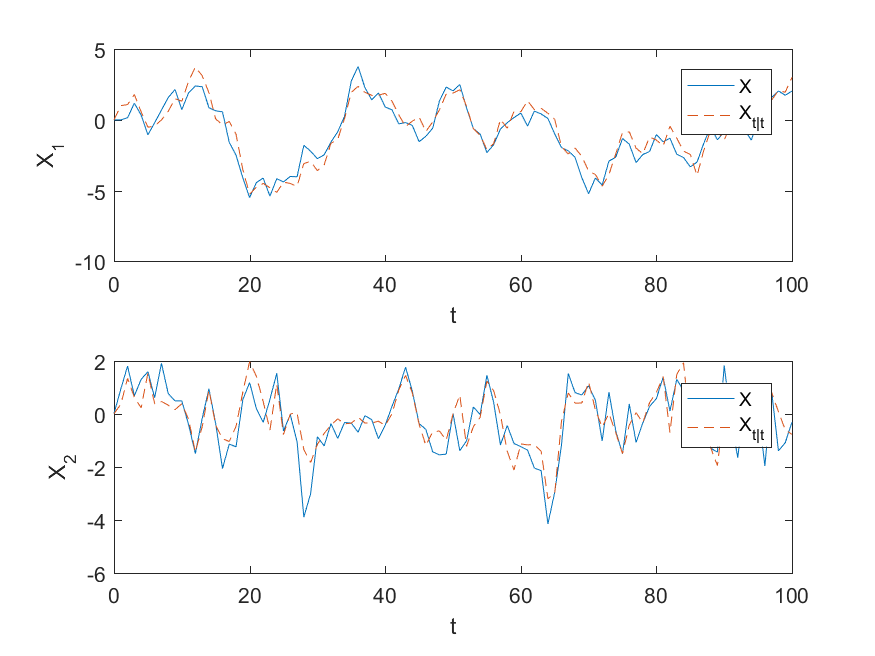
\includegraphics[width=.9\linewidth]{plot_c}
		\caption{Kalman filter estimate of $X_t$ for $T=100$.}
		\label{fig:plotc}
	\end{figure}
	\item

Note that 
	\[
	{\Sigma}_{X_t-X_{t\mid t}}  = P_{t\mid t} = 
	\pmat{0.5838 &  -0.0949\\
		-0.0949  &  0.5599}\]
	where $P_{t\mid t}$ is defined as in the notes. Note that in our particular case it is time invariant.

The sample covariance is given by
	\[
	\hat{\Sigma}_{X_t-X_{t\mid t}} 
	\pmat{ 0.5050  & -0.0734\\
		-0.0734   & 0.4794}\]
	
	Note that $\hat{\Sigma}_{X_t-X_{t\mid t}} $ and ${\Sigma}_{X_t-X_{t\mid t}}$ are really close to each other unlike previously with $\Sigma_X$, $\hat{\Sigma}_X$, $\Sigma_Z$ and $\hat{\Sigma}_Z$.
	
	\item
	\begin{enumerate}[(a)]
		\item
		
		See the code section. Note that we use the previous simulated series $X_t$.
		\item
	
	The variance of $Z$ is given by
		\[
		\sigma^2_Z = D\Sigma_XD' = 10.0183
		\]
		
		We can compute the sample variance of $Z$ and we get
		\[
		\hat{\sigma}_Z^2 =5.0167
		\]
		
		The discrepancy comes from the low number of data points, i.e. $T$.
		
		\item
		
		We plot the Kalman filter estimate $X_{t\mid t}$ in Figure \ref{fig:plote}.
		\begin{figure}[H]
			\centering
			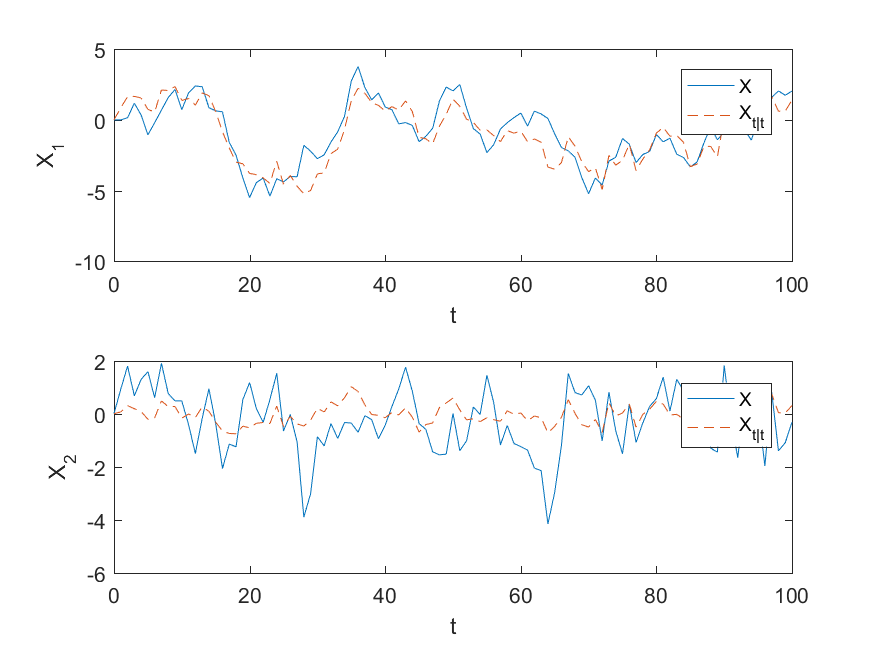
\includegraphics[width=.9\linewidth]{plot_e}
		\caption{Kalman filter estimate of $X_t$ for $T=100$.}
			\label{fig:plote}
		\end{figure}
	
	Note that we now have $Z_t=X_{1t}+X_{2t}$, while we previously had $Z_{1t}=X_{1t}+v_{1t}$ and $Z_2=X_{2t}+v_{2t}$. This implies that, while the observations of the first part of the problem were plagued with some extra error $v_t$ compare to $Z_t=X_{1t}+X_{2t}$, we did have twice the number of observations. This results in a better estimate of $X_t$ as shown in Figure \ref{fig:plotc}.
	
	But, even with only the sum of $X_{1t}$ and $X_{2t}$, Figure \ref{fig:plote} shows that the Kalman Filter still does a great job at retrieving $X_{1t}$ and $X_{2t}$.
	\end{enumerate}
	\item
	\begin{enumerate}[(a)]
		\item
		See the code section. Note that we use the previous simulated series $X_t$.
		
		\item
		
	The variance of $Z$ is given by
		\[
		\sigma^2_Z = D\Sigma_XD' =10.2564
		\]
		
		We can compute the sample variance of $Z$ and we get
		\[
		\hat{\sigma}_Z^2 = 4.4256
		\]
		
		The discrepancy comes from the low number of data points, i.e. $T$.
		
		\item
		
		We plot the Kalman filter estimate $X_{t\mid t}$ in Figure \ref{fig:plotf}.
		\begin{figure}[H]
			\centering
			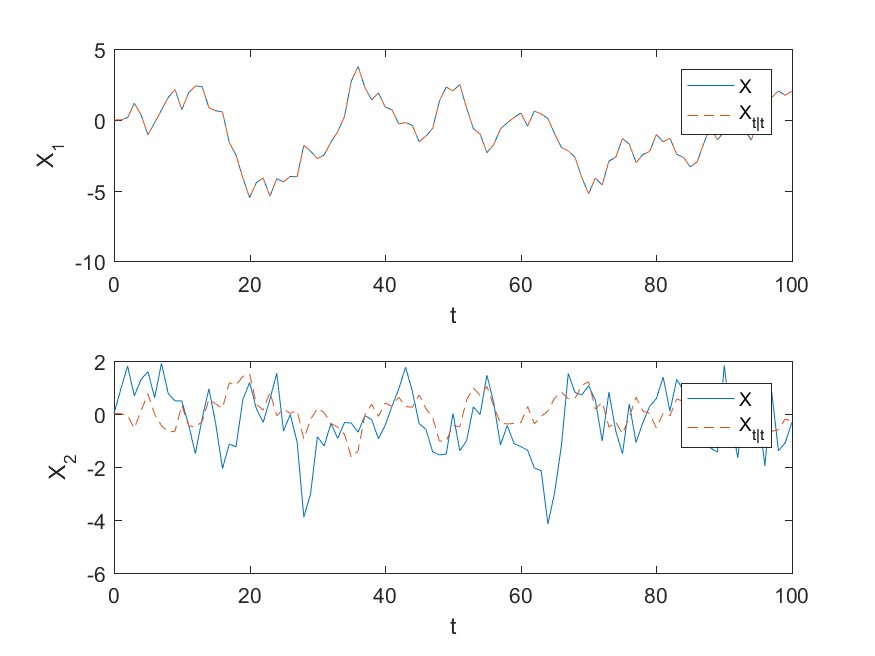
\includegraphics[width=.9\linewidth]{plot_f}
		\caption{Kalman filter estimate of $X_t$ for $T=100$.}
			\label{fig:plotf}
		\end{figure}
	
		Note that we now have $Z_t=X_{1t}$, while in part $Z_t=X_{1t}+X_{2t}$. Hence, we can perfectly determined $X_{1t}$ since $Z_t$ is noise free from anything else. Still even with no direct information about $X_{2t}$, the Kalman filter is still able to implicitly find a good estimate of $X_{2t}$.
	\end{enumerate}
\end{enumerate}

\section*{Code}\label{code}
\subsection*{main.m}
\lstinputlisting[language=Matlab]{main.m}
\subsection*{kfilter.m}
\lstinputlisting[language=Matlab]{kfilter.m}

\end{document}
